\chapter{Versuch 2}

\section{Benötigte Geräte}

Für dieses Experiment benötigen wir die Folgenden Geräte:
\begin{table}[h]	
	\centering
	\begin{tabular}[h]{c|c|c}
		Gerät & Anzahl & Produktbeeichnung\\
		\hline
		Oszilloskop & 1  & Keysight DSOX1102A\\
		\hline
		Frequenzgenerator & 1 & TELEDYNE T3AFG80\\
		\hline 
		Digital-Multimeter & 1 & Fluke TRUE RMS MULTIMETER\\
		\hline
		DAC & 1 & ZN429E \\
		\hline
		D-Flip-Flop & 1 & 
	\end{tabular}
	\caption{Materialliste Versuch 2}
	\label{tab:Materialliste Versuch 2}
\end{table}

\section{Versuchsaufbau}
\label{sec:Versuchsaufbau}
\begin{figure}[H]
	\centering
	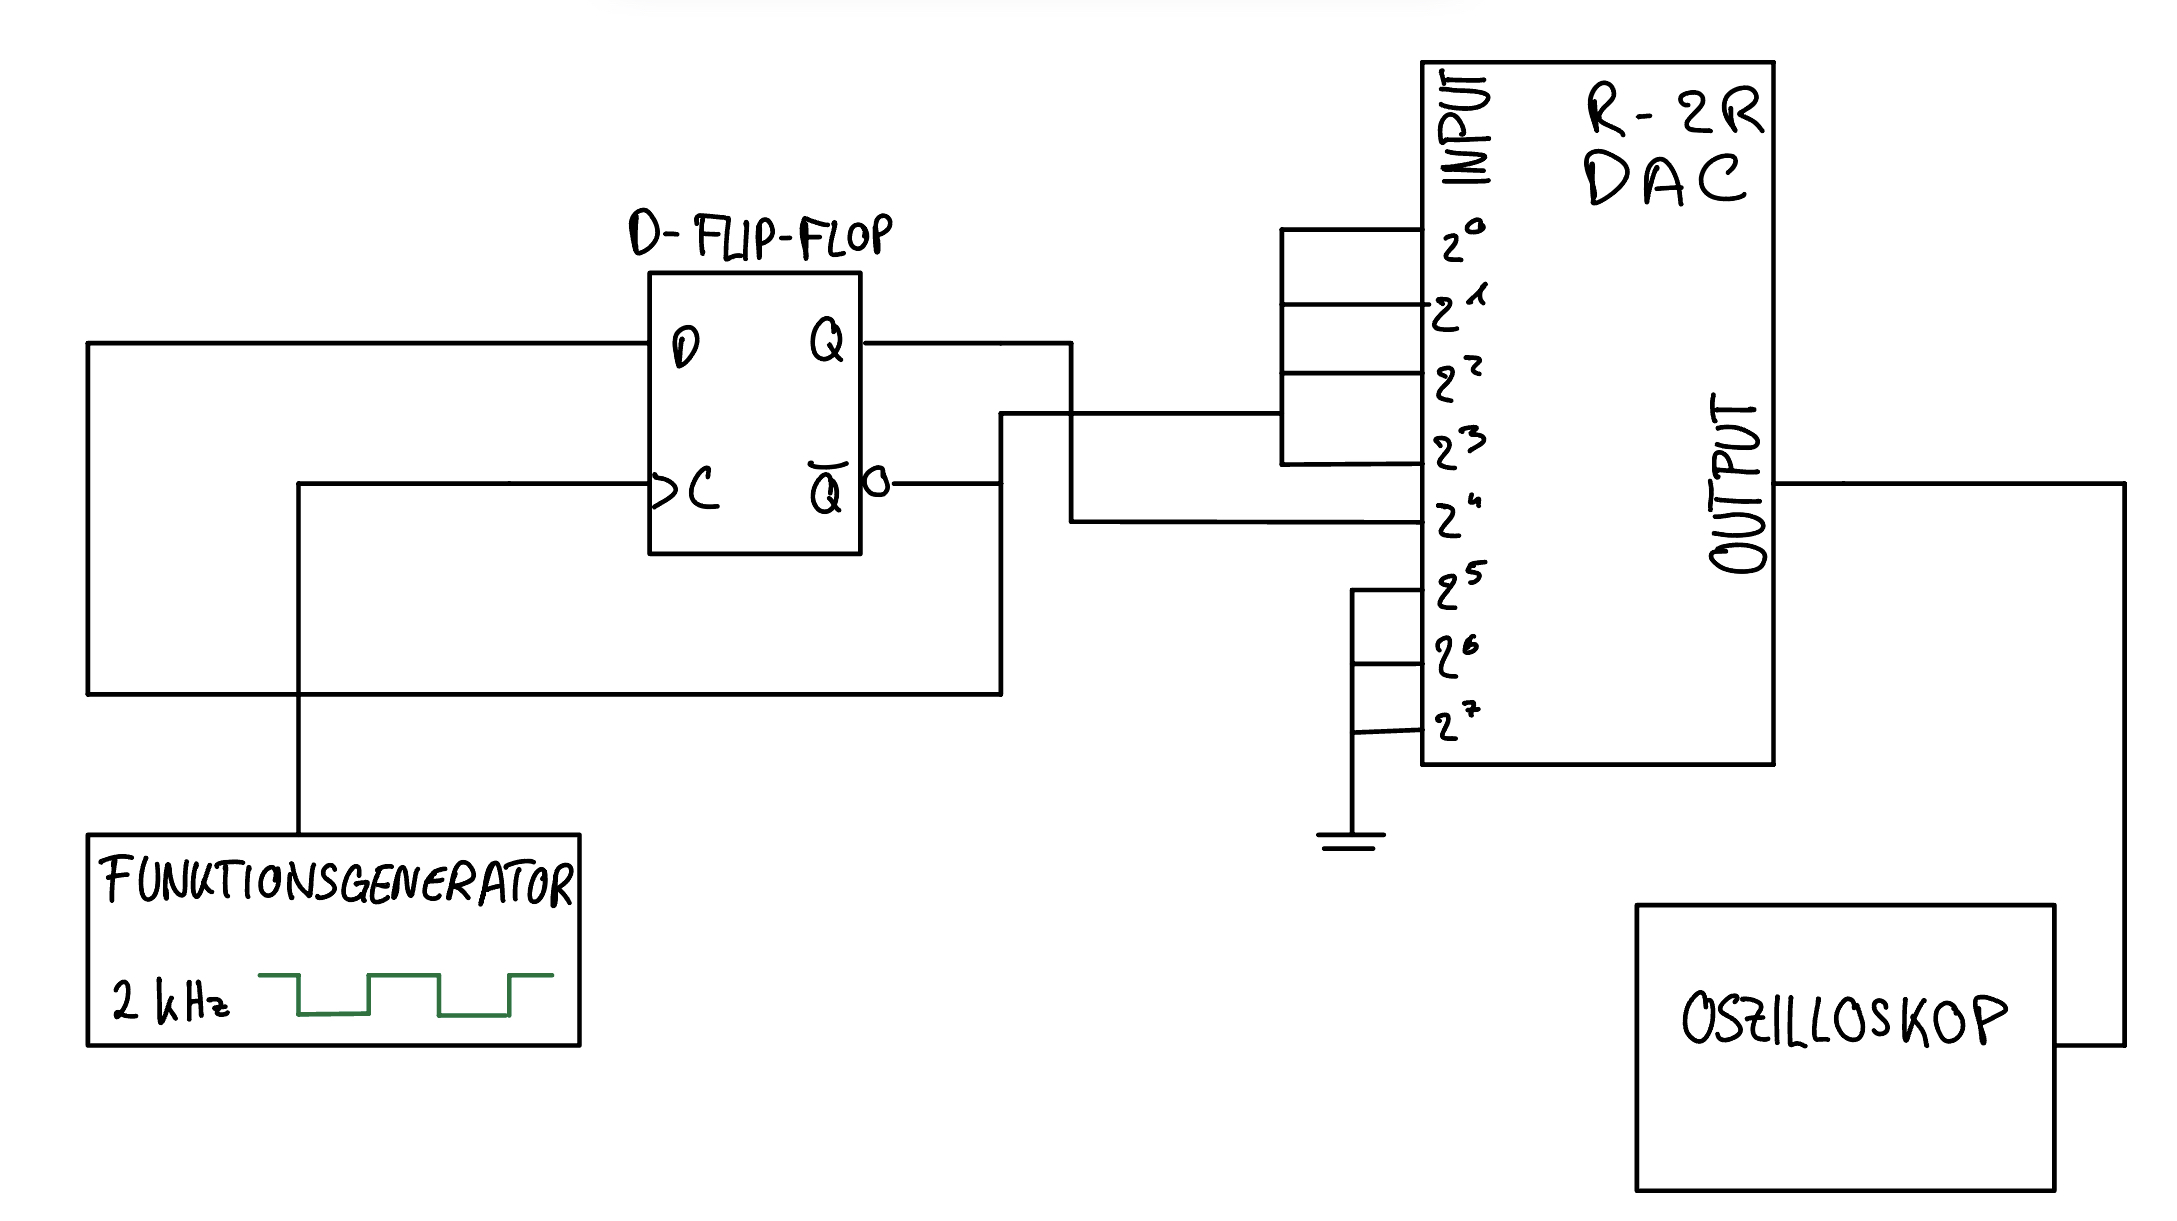
\includegraphics[height=7cm]{images/schaltungsskizze-versuch-zwei.jpeg} 
	\caption[]{Schaltungsskizze Versuch 2}
\end{figure}
Durch die Verbindung von $D\neg Q$ erreichet man eine aufsteigende Flanke
in einem Interval von 0,1ms. Hierbei ist zu beachten, dass $0,1ms \stackrel{^\wedge}{=} 1kHz$. 
Eine Halbierung der Frequenz im Vergleich zum Frequenzgenerator geschieht hier.

Der Spannungsberreich des DAC beträgt 0-2,55V, wobei 0V für 0000 0000 
und 2,55V für 1111 1111 steht. Ein LSB entspricht hierbei 10mV.

Die Referenzspannung kann aus dem Datenblatt abgelesen werden. Unter dem 
Parameter 'Full-scale output' ist eine Referenzspannung von 2,56V angegeben.

XXXXXXXXXXXXX Kondesator brauch man nicht.

\begin{figure}[H]
	\centering
	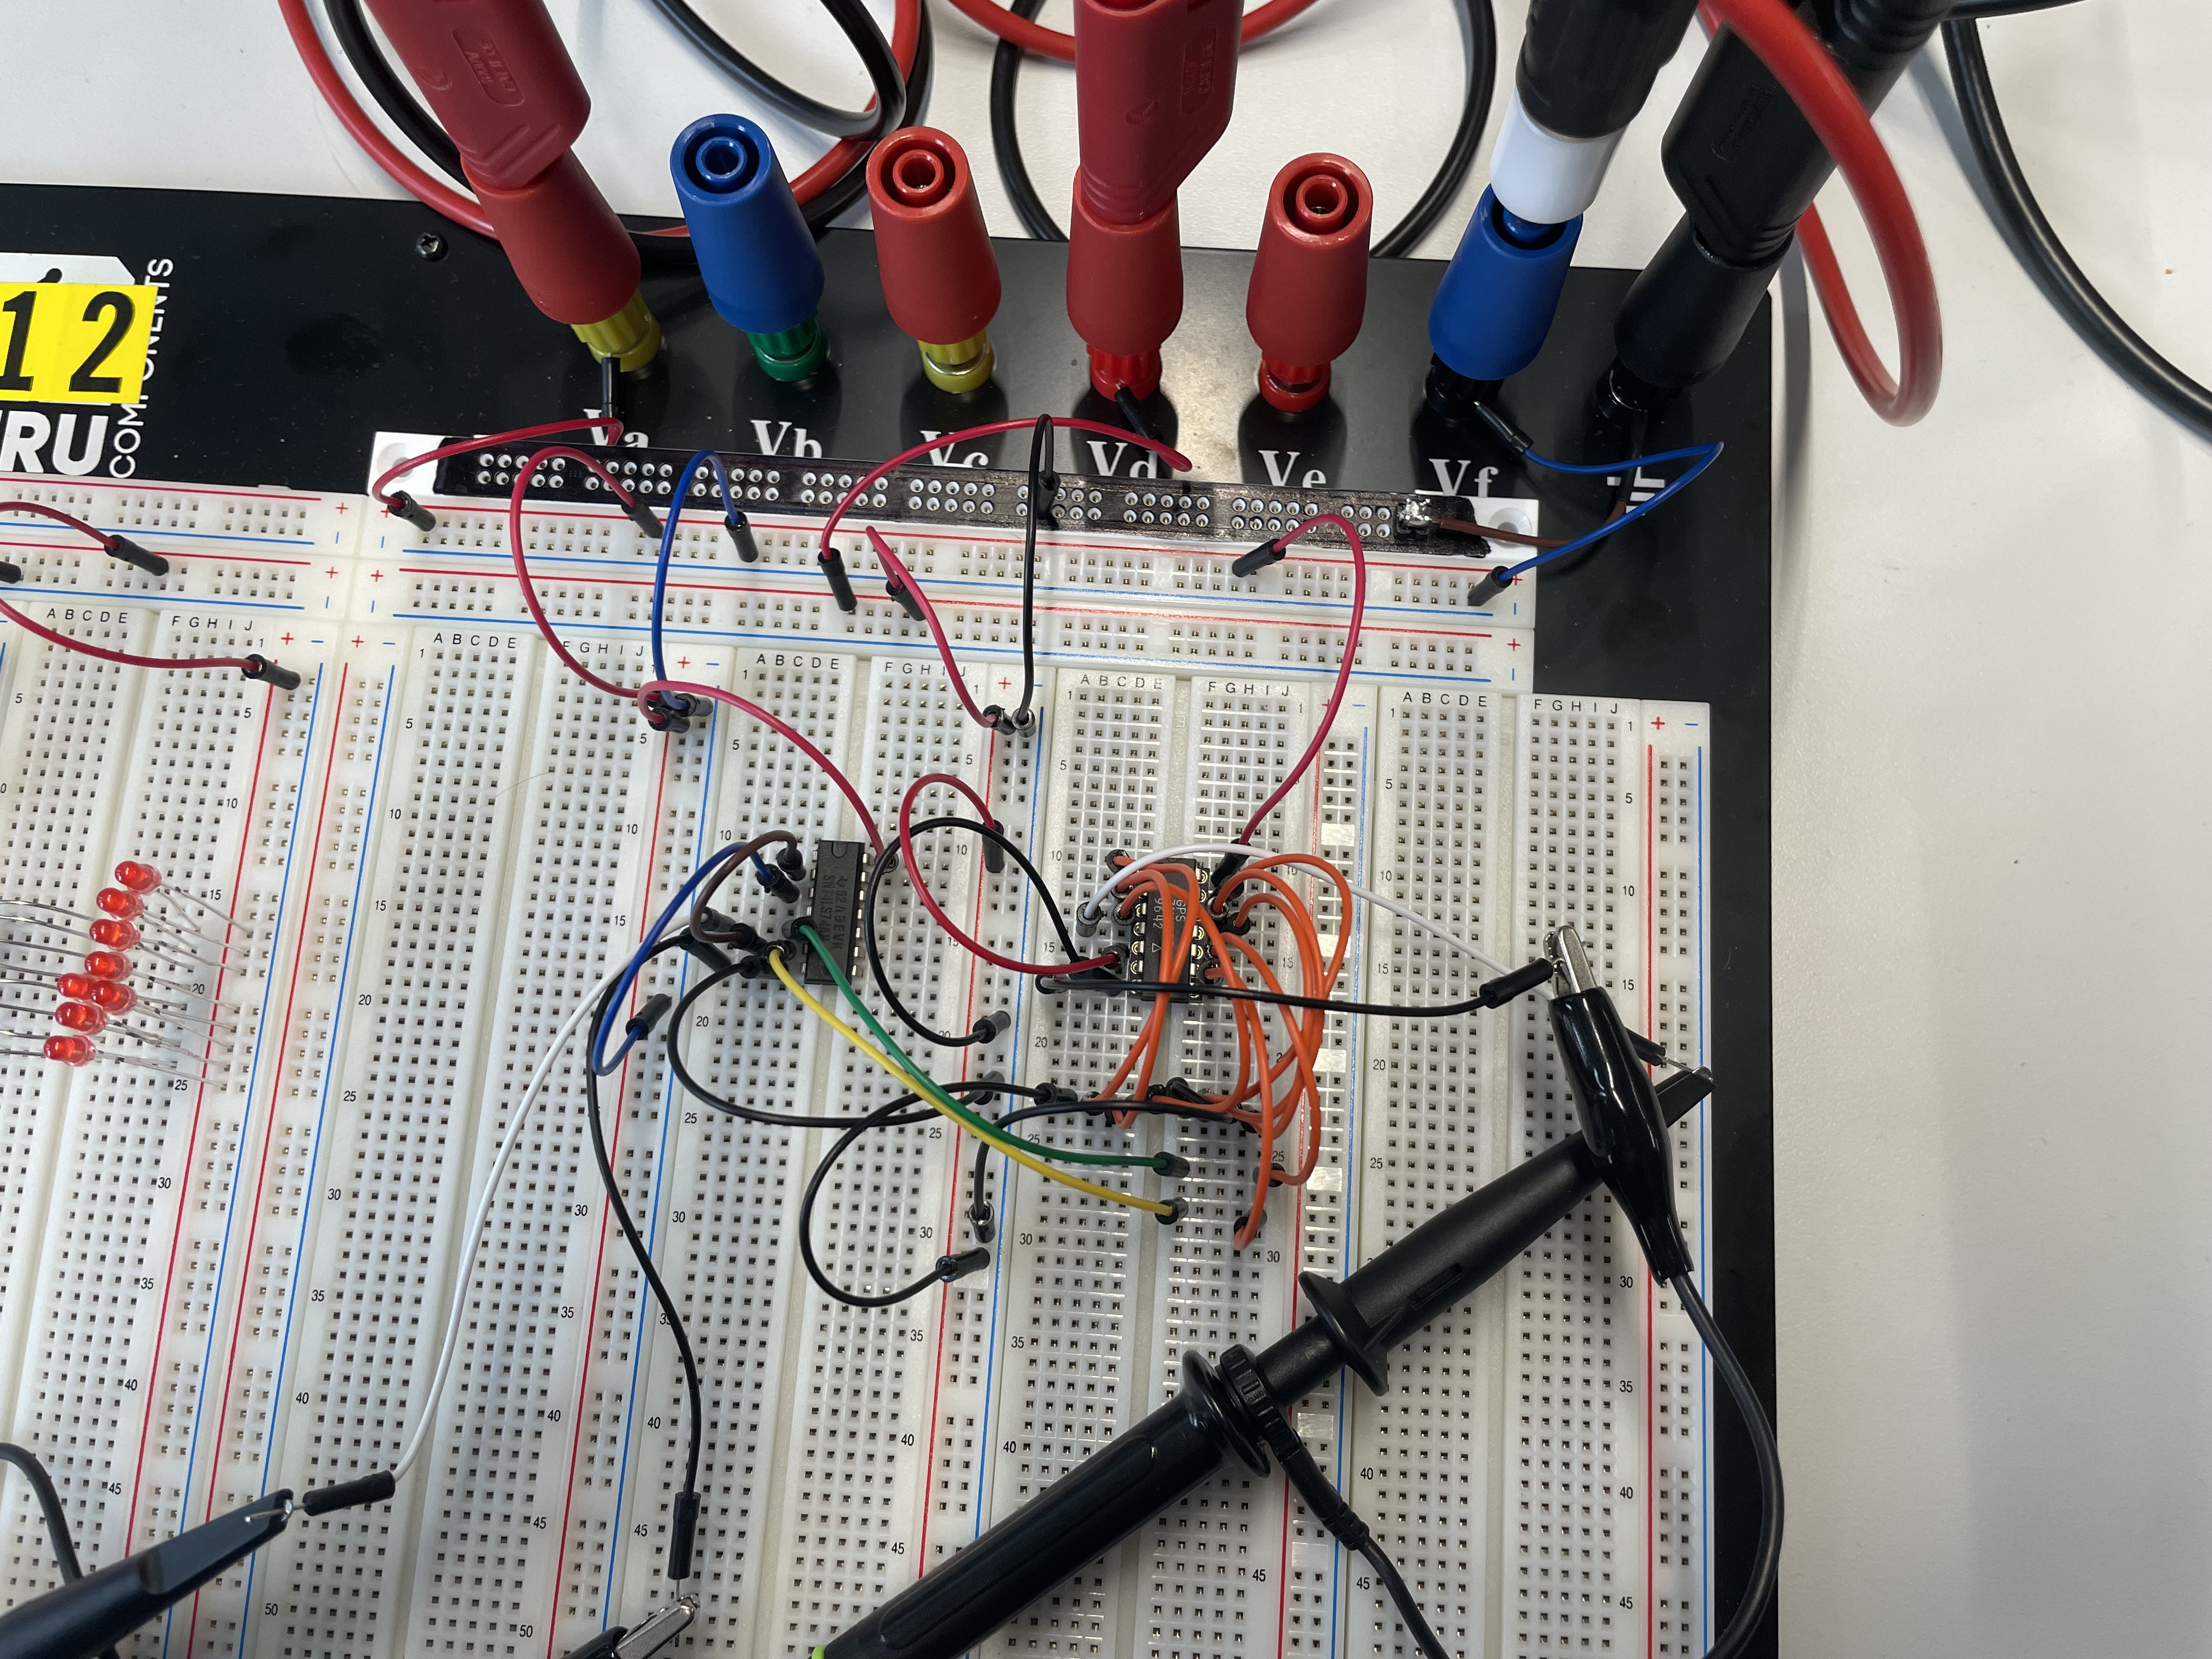
\includegraphics[height=7cm]{images/versuch2-schaltungsaufbau.jpeg} 
	\caption[]{Schaltungsaufbau Versuch 2}
\end{figure}



\section{Monotonie und Nichtlinearität}

\begin{figure}[H]
	\centering
	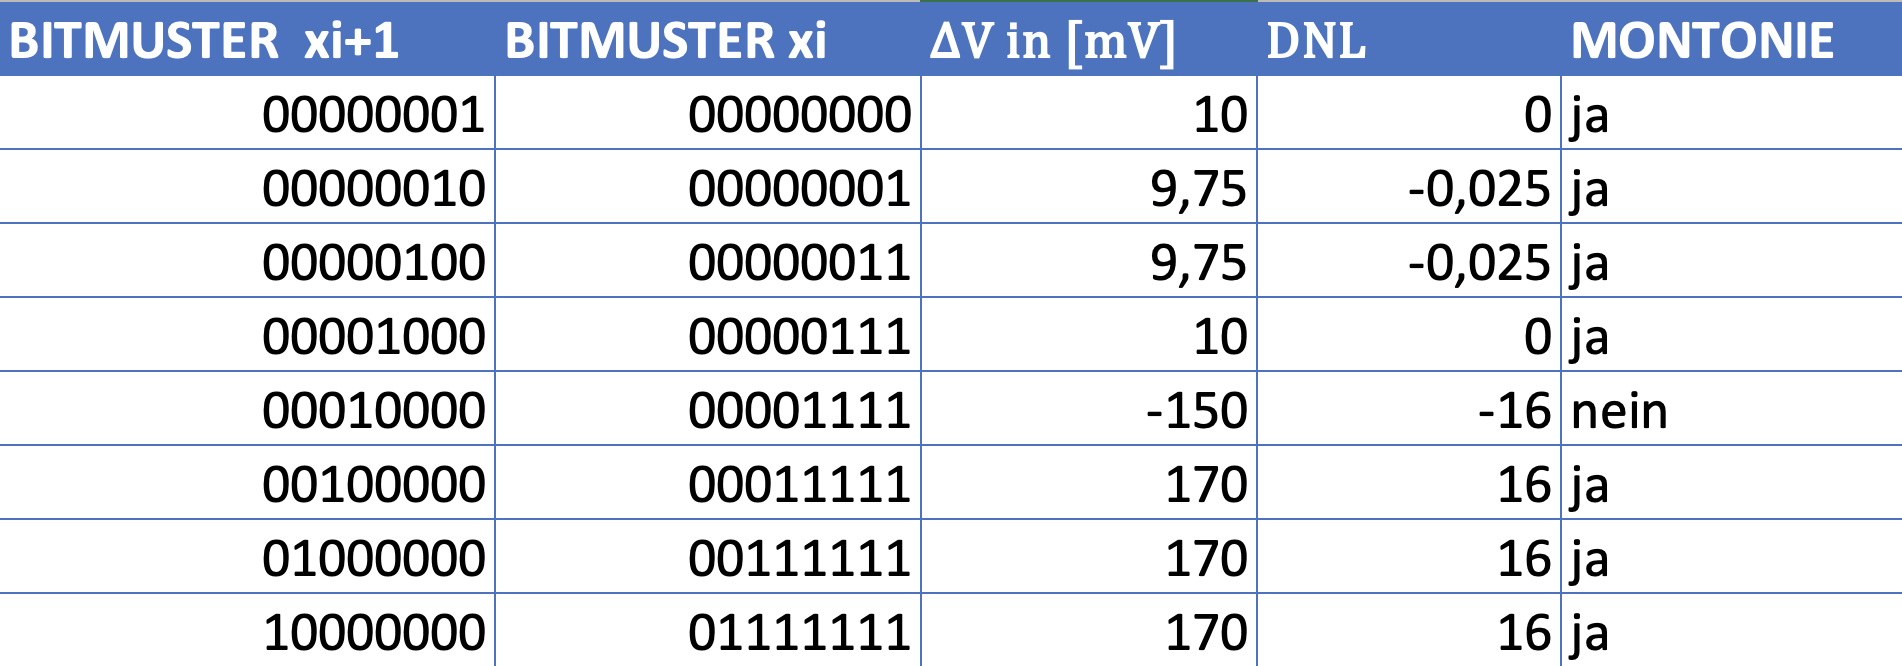
\includegraphics[height=5cm]{images/versuch2-monotonie-and-nichtlinearitaet.png} 
	\caption[]{Monotonieverhalten}
    \label{fig: Monotonieverhalten}
\end{figure}

Zu Vergleichen ist 
\[
\sum_{n=0}^{7} 2^n
\]
jeweils mit 
\[
\sum_{n=0}^{7} 2^n -1
\] als entsprechenden binärer Wert (siehe Abbildung \ref{fig: Monotonieverhalten})\newline
Unseren Ergebnissen kann man entnehmen, dass der DAC nicht
monoton ist. Bei genauerer Betrachtung fällt auf, dass das 5.
Bit kaputt ist und keine Spannung ausgibt. Grund hierfür ist 
vermutlich ein Versagen des Schalters im R-2R DAC.
Bei den nachfolgend getesteten Bitsprüngen sieht man, dass zu den
10 mV des eigentlichen Bitsprungs noch 160 mV hinzukommen, da 0001 0000
genau 160 mV entspricht.

Ein LSB entspricht wie in Kapitel \ref{sec:Versuchsaufbau} beschrieben 10mV.

Aus dem Datenblatt kann man ablesen, dass die Ausgangsimpedanz vom
DAC 10k$\Omega$ beträgt. Aufgrund einer so hohen Ausgangsimpedanz 
können Spannungsabfälle auftreten welche zu Signalverlusten führen 
könnten. Des weiteren können nachgeschaltene Bauteile mit niedriger
Eingangsimpedanz Signalverluste erleiden.




\section{Einschwingverhalten}

Zunächst einmal wurde der defekte DAC ausgetauscht 
gegen einen voll-funktionsfähigen. \newline
Die Frequenz der Alternierung des Flip-Flops ändert man zunächst nicht. \newline
Zum messen des Einschwingverhaltens legt man 2 Bitsprünge fest.
Einerseits den Bitsprung von 0000 0000 -> 0000 0001 und andererseits 
den Bitsprung von 0000 0000 -> 1111 1111.
Diese Werte eigenen sich gut, da hier im Datenblatt vom Hersteller 
zwei Referenzwerte gegeben sind, welche man nun zum Vergleich verwenden kann.\newline
Als Scope am Oszilloskop stellt man 200ns/div ein. \newline

\begin{table}[h]
	\centering
	\begin{tabular}[h]{c|c|c|c}
		Bitsprung & 90\% [in ns] & 100\% [in ns] & Angabe Datenblatt [in ns] \\
		\hline
		00000 0000 -> 0000 0001 & 540 & 1592 & 1000\\
		\hline
		0000 0000 -> 1111 1111 & 830 & 1448 & 2000\\
	\end{tabular}
	\caption{Einschwingverhalten in Prozent}
	\label{tab:Einschwingverhalten}
\end{table}

Die Abweichung zum Datenblatt liegt hier im gewöhnlichen Bereich.
Die genauen Ausmessungen vomn Oszilloskop sind im Anhang A bis D zu finden.
Allerdings ist es hier fragwürdig, warum die Einschwingzeit für 100\% in der
zweiten Versuchsreihe kürzer ist als in der ersten. Dies liegt vermutlich an
einem Messfehler. \newline 


